\documentclass[11pt,letterpaper]{article}
\usepackage[lmargin=1in,rmargin=1in,tmargin=1in,bmargin=1in]{geometry}
\usepackage{../style/homework}
\usepackage{../style/commands}
\setbool{quotetype}{false} % True: Side; False: Under
\setbool{hideans}{false} % Student: True; Instructor: False

% -------------------
% Content
% -------------------
\begin{document}

\homework{7: Due 03/01 (02)}{Take chances, make mistakes. That's how you grow. Pain nourishes your courage. You have to fail in order to practice being brave.}{Mary Tyler Moore}

% Problem 1
\problem{10} Being as detailed as possible, answer the following:
	\begin{enumerate}[(a)]
	\item What are two measures of `center' for a dataset? 
	\item What are two measures of `variability' for a dataset?
	\item Name a measure of center which is robust and a measure of center which is not robust. 
	\end{enumerate} \pspace

\sol 
\begin{enumerate}[(a)]
\item There are many notions of `center.' Among the more common measures of center are mean, median, midrange, etc. \pspace

\item There are many notions of `variability' for a data set. Among the more common measures of variability are standard deviation, IQR, and range. \pspace

\item The median is a measure of center which is robust while the mean is a measure of center which is not robust. For instance, given the dataset 1, 2, 3, both the median and mean are 2. However, if the outlier 100 is added, the median changes to 2.5 while the mean changes to 53. 
\end{enumerate}



\newpage



% Problem 2
\problem{10} Stewart is tracking snowfall received over the past few days in his area. He finds the following number of inches of snow has fallen over the past few days:
	\[
	1.5" \qquad 4.2" \qquad 0" \qquad 0.8" \qquad 5.1"
	\]

\begin{enumerate}[(a)]
\item Find the mean inches of snow that fell this week.
\item Find the standard deviation for the this week's snowfall. 
\item If Stewart underestimated the inches that fell each day by 0.5", what would be the average snowfall for the week?
\end{enumerate} \pspace

\sol 
\begin{enumerate}[(a)]
\item We have\dots
	\[
	\overline{x}= \dfrac{1.5" + 4.2" + 0" + 0.8" + 5.1"}{5}= \dfrac{11.6"}{5}= 2.32"
	\] \pspace

\item We have\dots \par
	\begin{table}[!ht]
	\centering
	\begin{tabular}{r|r|r}
	$x_i$ & $x_i - \overline{x}$ & $(x_i - \overline{x})^2$ \\ \hline
	$1.5$ & $-0.82$ & $0.6724$ \\
	$4.2$ & $1.88$ & $3.5344$ \\
	$0$ & $-2.32$ & $5.3824$ \\
	$0.8$ & $-1.52$ & $2.3104$ \\
	$5.1$ & $2.78$ & $7.7284$ \\ \hline
	& Total: & 19.6280
	\end{tabular}
	\end{table} \par
Therefore, we have\dots
	\[
	s^2= \dfrac{1}{n - 1} \sum (x_i - \overline{x})^2= \dfrac{1}{5 - 1} \cdot 19.6280= \dfrac{19.6280}{4}= 4.807
	\]
But then we have $s= \sqrt{s^2}= \sqrt{4.807} \approx 2.192"$. \pspace

\item Because each day's snowfall is 0.5" less, we anticipate the average snowfall is 0.5" less than what was computed in (a). But then we have $\overline{x}= 2.32" - 0.5"= 1.82"$. We can confirm this with a direct computation:
	\[
	\overline{x}= \dfrac{1.0" + 3.7" - 0.5" + 0.3" + 4.6"}{5}= \dfrac{9.1"}{5}= 1.82"
	\]
\end{enumerate}



\newpage



% Problem 3
\problem{10} Charlie is at a town hall meeting. He goes around the room and asks each person their age. Charlie finds the following responses for the ages of the people at the meeting:
	\[
	66 \qquad 50 \qquad 67 \qquad 40 \qquad 70 \qquad 56 \qquad 69 \qquad 57 \qquad 40 \qquad 44
	\]

\begin{enumerate}[(a)]
\item Find the median for this dataset. 
\item Find the IQR for this dataset.
\item Sketch a box and whisker plot for this dataset. 
\end{enumerate} \pspace

\sol 
\begin{enumerate}[(a)]
\item Ordering the data, we have\dots
	\[
	40 \qquad 40 \qquad 44 \qquad 50 \qquad 56 \qquad 57 \qquad 66 \qquad 67 \qquad 69 \qquad 70
	\]
There are 10 numbers. Therefore, because $\frac{10}{2}= 5$, the median is the average of the 5th and 6th number. Then the median is $\frac{56 + 57}{2}= \frac{113}{2}= 56.5$. \pspace

\item The numbers less than this median are 40, 40, 44, 50, and 56. The median of these numbers is 44. But then $Q_1= 44$. The numbers greater than 56.5 are 57, 66, 67, 69, and 70. The median of these numbers is 67. But then $Q_3= 67$. Therefore, we have\dots
	\[
	\text{IQR}= Q_3 - Q_1= 67 - 44= 23
	\] \pspace

\item Observe that $1.5 \text{IQR}= 1.5 \cdot 23= 34.5$. We now have $Q_1 - 1.5 \text{IQR}= 44 - 34.5= 9.5$ and $Q_3 + 1.5\text{IQR}= 67 + 34.5= 101.5$. The box and whisker plot is then\dots
	\[
	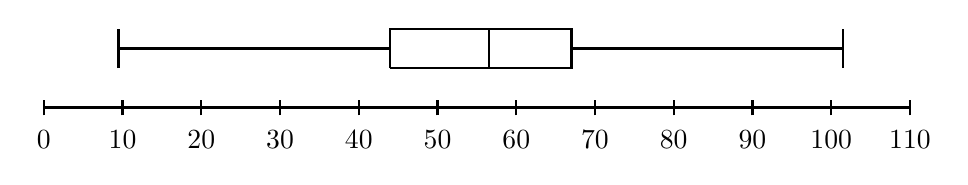
\begin{tikzpicture}
	\draw[line width= 0.03cm] (0,0) -- (11,0);
	\foreach \x [evaluate=\x as \themark using \x/10] in {0,10,...,110} {
	\draw[line width=0.03cm] (\themark,-0.1) -- (\themark,0.1);
	\node at (\themark,-0.4) {\x};
	}
	\draw[line width=0.03cm] (4.4,0.5) -- (4.4,1) -- (6.7,1) -- (6.7,0.5) -- (4.4,0.5);
	\draw[line width=0.03cm] (5.65,0.5) -- (5.65,1);
	\draw[line width=0.03cm] (0.95,0.5) -- (0.95,1);
	\draw[line width=0.03cm] (0.95,0.75) -- (4.4,0.75);
	\draw[line width=0.03cm] (6.7,0.75) -- (10.15,0.75);
	\draw[line width=0.03cm] (10.15,0.5) -- (10.15,1);
	\end{tikzpicture}
	\]
\end{enumerate}



\newpage



% Problem 4
\problem{10} Lorelei is finding the mean of the numbers 17, 18, 26, 19. She finds that the mean is 40. By comparing Lorelei's mean as a measure of `center' to the size of the numbers, how would you explain to her why this cannot be correct. What has Lorelei done incorrectly? How would you explain to her how to fix her work? \pspace

\sol If the mean is a measure of `center', then it should be in the `center' of the numbers. However, 40 is much larger than all the listed numbers. Therefore, it should not be possible for 40 to be the `center' of these numbers. We know that\dots
	\[
	\overline{x}= \dfrac{\text{sum numbers}}{\text{amount of numbers}}= \dfrac{17 + 18 + 26 + 19}{4}= \dfrac{80}{4}= 20
	\]
Therefore, the correct mean is 20. We can see from this calculation that Lorelei likely did the following:
	\[
	\overline{x}= \dfrac{\text{sum numbers}}{2}= \dfrac{17 + 18 + 26 + 19}{2}= \dfrac{80}{2}= 40
	\]
Likely, this is a result of computing the mean of only two numbers many times and internalizing that to find the mean you find the sum of the numbers and divide by 2. 


\end{document}